<<<<<<< HEAD
% Time-stamp: <2023-09-01 22:08:59 vladimir>
% Copyright (C) 2019-2023 Vladimir G. Ivanović
% Author: Vladimir G. Ivanović <vladimir@acm.org>
% ORCID: https://orcid.org/0000-0002-7802-7970
=======
%%% Time-stamp: <2023-07-18 11:03:25 vladimir>
% %%% Copyright (C) 2019-2023 Vladimir G. Ivanović
% %%% Author: Vladimir G. Ivanović <vladimir@acm.org>
% %%% ORCID: https://orcid.org/0000-0002-7802-7970

\begin{comment}
  \section{Charter School Financing}
    \subsection{Charter School Financial Documents}
      \subsubsection{Petitions \& Renewals}
      \subsubsection{Authorizer Staff Reports}
      \subsubsection{Budgets, Interim Reports, and CAFRs}
      \subsubsection{LCAPs,}
      \subsubsection{Board and Committee Supporting Material}
    
  \section{Charter Schools and Real Estate}
    \subsection{Facilities Options}
      \subsubsection{Co-Locating}
      \subsubsection{Leasing}
      \subsubsection{Owning}
    \subsection{Funding Facility Ownership}
      \subsubsection{Private Funding: Loans and Foundation Grants}
      \subsubsection{Venture Funds}
      \subsubsection{Tax Credits}
      \subsubsection{Bonds}
    
  \section{Other Data}
    \subsection{Datasets}
    \subsection{State and Federal Filings}
    \subsection{Curated Social Media}
  
  \section{Gaps and Anomalies}
    \subsection{Triangulation}
\end{comment}
>>>>>>> 4685233 (Fixups to 'methods.tex'.)

\chapter{Findings}\label{ch:findings}\noindent
\todo{Rocketship expansion criteria}
\todo{Rockethip has expanded into Redwood City, Antioch, and San Francisco}
\todo{Rocketship expanded into Wisconsin, Tennessee, and Washington, D.C., and they wanted to expand into Texas. Is there anything special about these locations that make them especially favorable? State law? State board of education? Demographic considerations? Influence of major charter school proponents and donors?}
\todo{Has Rocketship not expanded into some locations because of existing charter schools?}
\todo{What's with joining the El Dorado County SELPA? }
\todo{What is a plausible exit strategy?}
\todo{Keep track of people and cross-reference with LittleSis}
\todo{Keep track of ways that Rocketship has cut costs using the data in petitions}
\todo{Track down the origin of "held in trust" comment in the 2022 CSFA presentation
- Presentation: Charter School Facilities Program 2022 Filing Round: Informational Webinar, 01 Mar 2023
- See [p. 29] May 2 – June 3: California School Finance Authority: Program Overview
- What does this mean? Where is it specified?}

This chapter presents the data found using the approach outlined in \prettyref{ch:methods} with the goal of answering my research question: Has Rocketship structured itself and its finances, to earn a return to investors, focusing especially on real estate transactions, and if so, how?

Since real estate is so important for Rocketship, the next section, \prettyref{sec:location-and-property-info} will lay out what facilities Rocketship has, where those facilities are located, when they were acquired, and what real estate rights Rocketship has over those properties.

<<<<<<< HEAD
=======
%%%%%%%%%%%%%%%%%%%%%%%%%%%%%%%%%%%%%%%%%%%%%%%%%%%%%%%%%%%%%%%%%%%%%%%%%%%%%%%
%%% Rocketship History %%%
%%%%%%%%%%%%%%%%%%%%%%%%%%%%%%%%%%%%%%%%%%%%%%%%%%%%%%%%%%%%%%%%%%%%%%%%%%%%%%%
\section{Rocketship History}\label{sec:history}\indent

\subsection{Rocketship's Corporate Structure}\label{sec:RSED-corporate-structure}\indent

Rocketship's corporate structure was designed from the start to separate schools and their operation from facilities and their construction and maintenance. Rocketship Education is the parent company, a 501(3)(c) non-profit. It owns all the schools, themselves non-profits, plus Launchpad Development Company, another non-profit. Launchpad Development's role is to own all the facilities, one non-profit LLC per location. This structure is diagrammed in \prettyref{fig:RSED-corporate-structure}.

\begin{enumerate}
  \item Articles of Incorporation
\end{enumerate}
\subsection{Launchpad Development LLC}
\begin{enumerate}
  \item Articles of Incorporation
\end{enumerate}

\begin{figure}[ht]
  \centering
  \caption{\normalfont\emph{Rocketship's Corporate Structure (Santa Clara County only) Schools}}\label{fig:corporate-structure}\label{fig:corporate-structure}
  \sffamily
  \begin{forest}
    for tree={grow'=east, folder, draw, align=left}
    [ \textbf{Rocketship Education}, baseline
      [ Launchpad Development Company
        [ \textit{Launchpad (LP)}, xshift=4em ]
        [ \textit{Launchpad Development One LLC (LLC1)}, xshift=4em ]
        [ \textit{Launchpad Development Two LLC (LLC2)}, xshift=4em ]
        [ \textit{Launchpad Development Threee LLC (LLC3)}, xshift=4em ]
        [ \textit{Launchpad Development Four LLC (LLC4)}, xshift=4em ]]
      [ Rocketship Support Network (RSN) ]
      [ Rocketship Mateo Sheedy Elementary (RSM) ]
      [ Rocketship Sí-Se-Puede Academy (RSSP) ]
      [ Rocketship Mosaic Elementary (ROMO) ]
      [ Rocketship Discovery Prep (RDP) ]
      [ Rocketship Brilliant Minds (RBM) ]
      [ Rocketship Alma Academy (RSA) ]
      [ Rocketship Spark Academy (RSK) ]
      [ Rocketship Rising Stars (RRS) ]]
    \end{forest}
  \end{figure}

%%%%%%%%%%%%%%%%%%%%%%%%%%%%%%%%%%%%%%%%%%%%%%%%%%%%%%%%%%%%%%%%%%%%%%%%%%%%%%% 
%%% Rocketship Budgets
%%%%%%%%%%%%%%%%%%%%%%%%%%%%%%%%%%%%%%%%%%%%%%%%%%%%%%%%%%%%%%%%%%%%%%%%%%%%%%%
\begin{figure}
  \centering
  \caption[Financial Statements Collected]{\textit{Financial Statements Collected}} \label{fig:financial-statements-collected}
 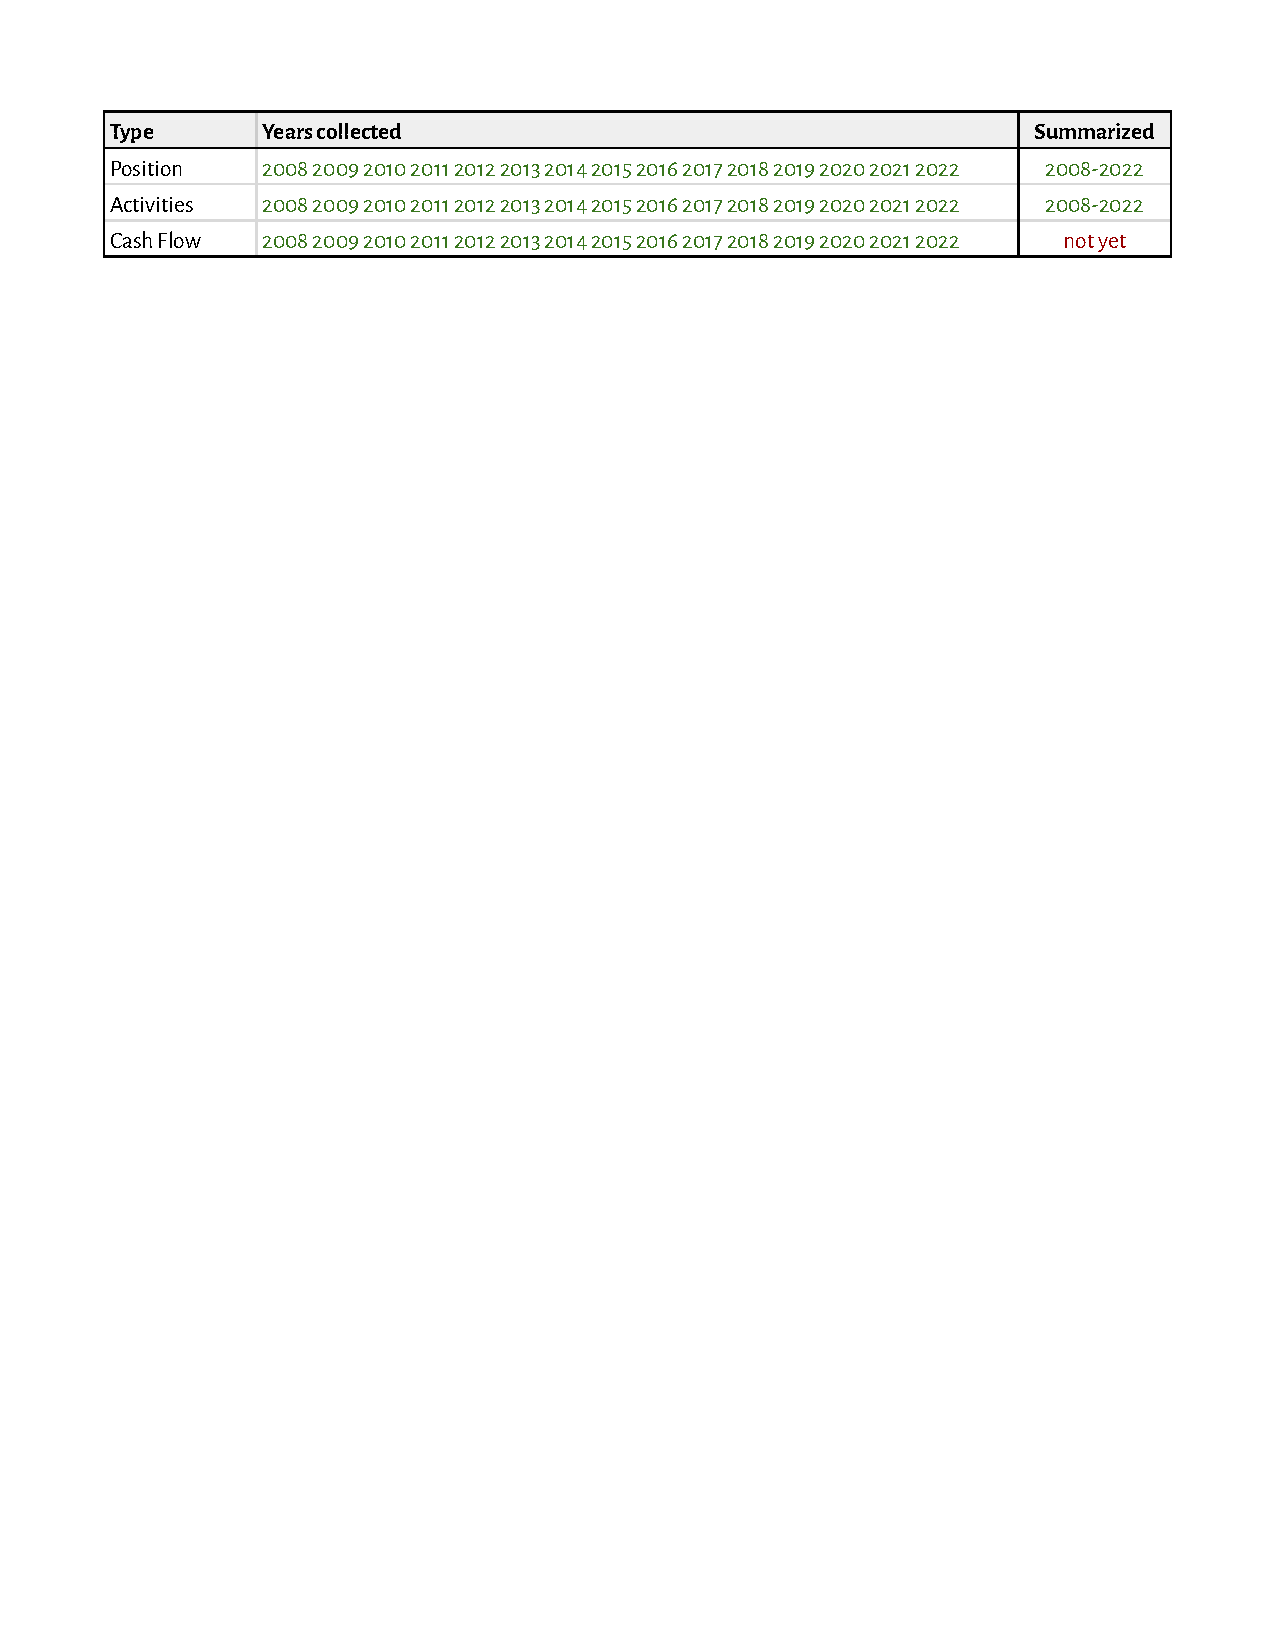
\includegraphics[width=\textwidth]{Consolidated_Financial_Statements/Financial_Statements_Collected_Summarized.pdf}\\ %chktex 8
\end{figure}
    
%%%%%%%%%%%%%%%%%%%%%%%%%%%%%%%%%%%%%%%%%%%%%%%%%%%%%%%%%%%%%%%%%%%%%%%%%%%%%%% 
%%% Rocketship Properties
%%%%%%%%%%%%%%%%%%%%%%%%%%%%%%%%%%%%%%%%%%%%%%%%%%%%%%%%%%%%%%%%%%%%%%%%%%%%%%%
>>>>>>> 4685233 (Fixups to 'methods.tex'.)
\section{Rocketship Locations and Property Information}\label{sec:location-and-property-info}\indent

\begin{table}[hbt]
  \caption[Rocketship Property Information]{\textit{Rocketship Property Information}}\label{tab:locations}\SingleSpacing%
  \begin{tabular}{lll}
    \toprule
    School          & Address                               & Property Information \\
    \midrule
    Mateo Sheedy    & 788 Locust St., San José, CA 95110    & \prettyref{sec:mateo-sheedy-info} \\
    Sí Se Puede     & 2249 Dobern Ave, San José, CA 95116   & \prettyref{sec:sí-se-puede-info} \\
    Los Sueños      & 331 S. 34th St, San José, CA 95116    & \prettyref{sec:los-suenos-info} \\
    Discovery Prep  & 370 Wooster Ave, San José, CA 95116   & \prettyref{sec:discover-prep-info} \\
    Mosaic          & 950 Owsley Ave, San José, CA 95122    & \prettyref{sec:mosaic-info} \\
    Brilliant Minds & 2960 Story Rd, San José, CA 95127     & \prettyref{sec:brilliant-minds-info} \\
    Alma Academy    & 198 West Alma Ave, San José, CA 95110 & \prettyref{sec:alma-academy-info} \\
    Spark Academy   & 683 Sylvandale Ave San José, CA 95111 & \prettyref{sec:spark-academy-info} \\
    Fuerza          & 70 S. Jackson Ave, San José, CA 95116 & \prettyref{sec:fuerza-info} \\
    Rising Stars    & 3173 Senter Road, San José, CA 95111  & \prettyref{sec:rising-stars-info} \\
    \bottomrule
  \end{tabular}
\end{table}

This chapter presents data found using the approach outlined in \prettyref{ch:methods} with the goal of answering my research question: Has Rocketship structured itself and its finances, to earn a return to investors, focusing especially on real estate transactions, and if so, how?

The first section will give a short historical overvew of Rocketship in \prettyref{sec:history}, including a section on how Rocketship has structured itself. 

Since real estate is so important for Rocketship, the next section, \prettyref{sec:location-and-property-info} will lay out what facilities Rocketship has, where those facilities are located, when they were acquired, and what real estate rights Rocketship has over those properties.

\subsection{Rocketship's Corporate Structure}\label{sec:rocketship-corp-struct}\indent

Rocketship's corporate structure was designed from the start to separate schools and their operation from facilities and their construction and maintenance. Rocketship Education, Inc. is the parent company, a 501(3)(c) non-profit. It owns all the schools, themselves non-profits, plus Launchpad Development Company, another non-profit. Launchpad Development's role is to own all the facilities, one non-profit LLC per location. This structure is diagrammed in \prettyref{fig:RSED-corporate-structure}.

\begin{figure}[h]
  \centering
  \caption{\normalfont\emph{Rocketship's Corporate Structure (Santa Clara County only)}}\label{fig:RSED-corporate-structure}
  \sffamily
  \begin{forest}
    for tree={grow'=east, folder, draw, align=left}
    [ \textbf{Rocketship Education}, baseline
    [ Launchpad Development Company
    [ \textit{Launchpad (LP)}, xshift=4em ]
    [ \textit{Launchpad Development One LLC (LLC1)}, xshift=4em ]
    [ \textit{Launchpad Development Two LLC (LLC2)}, xshift=4em ]
    [ \textit{Launchpad Development Threee LLC (LLC3)}, xshift=4em ]
    [ \textit{Launchpad Development Four LLC (LLC4)}, xshift=4em ]]
    [ Rocketship Support Network (RSN) ]
    [ Rocketship Mateo Sheedy Elementary (RSM) ]
    [ Rocketship Sí-Se-Puede Academy (RSSP) ]
    [ Rocketship Mosaic Elementary (ROMO) ]
    [ Rocketship Discovery Prep (RDP) ]
    [ Rocketship Brilliant Minds (RBM) ]
    [ Rocketship Alma Academy (RSA) ]
    [ Rocketship Spark Academy (RSK) ]
    [ Rocketship Rising Stars (RRS) ]]
  \end{forest}
\end{figure}

\section{Charter School Financing}\label{sec:findings-charter-financing}\indent

Financing charter schools in California is more complicated than the financing of traditional public schools because charters need to obtain facilities, often independently from the public school district in which they are located.
 \prettyref{tab:charter-financing-options} describes what financing options a charter school has compared to a traditional public school.

\subsection{Charter School Financing Options}\indent\label{sec:charter-school-financing-options}

\begin{table}[thb]
  \caption[Charter School Financing Options]{\textit{Charter School Financing Options}}\label{tab:charter-financing-options}%
  \SingleSpacing%
  \begin{tabular}{lccl}
    \toprule
    Type             & \multicolumn{2}{c}{Available to}  & Notes\\
                         & TSPs & Charters                   & \\
    \midrule
    LCFF                 & Yes  & Yes                        & Minimum state guarantee, per ADA\\ 
    Local property tax   & Yes  & Yes                        & Reduces LCFF amount\\
     & & &\\ % Empty row as a divider
    Categorical programs & Yes  & Yes                        & \multirow[t]{2}{3in}{All federal funding is categorical,\\
                                                               as is all state funding outside of LCFF}\\
    \\
    Local parcel tax     & Yes  & No                         & Established by district election\\
    Revenue bonds        & Yes  & Yes                        & \multirow[t]{2}{3in}{TSPs: district election\\
                                                               Charters: private placement only}\\
    \\
    Construction loans   & Yes  & Yes                        & \multirow[t]{2}{3in}{Federal, state, \& private loans\\
                                                               with widely varing terms}\\
    \\
    COVID-19 PPP loans   & N/A & Yes                         & Paycheck Protection Program loan → grant\\
    Venture fund loans   & No  & Yes                         & Often using New Market Tax Credit program\\
    Private grants       & Yes & Yes                         & Much more common with charters\\
    Rent subsidies       & No  & Yes                         & SB740\\
 \bottomrule
  \end{tabular}
\end{table}
The first two sources of financing, i.e.~revenue, are always available to both public schools and to charter schools, although the amounts and timing of the distributions might vary.

\begin{description}[nosep]\OnehalfSpacing%
  \medskip\item[LCFF] Local Control Funding Formula. A charter's home district passes through an amount based on a school's demographics and ADA (Average Daily Attendance). All schools have the same base grant adjusted for grade spans.  If a school has students who are low income (i.e.~they are eligible for free or reduced price meals (FRPM)), or they are English Learners (EL), or they are foster youth, the school receives a supplemental grant of 20\% of its adjusted base grant. If the qualifying population of students exceeds 55\% of the total, a school receives 65\% of the adjusted base grant for every student above the 55\% threshold.

Since all Rocketship schools have at least 55\% of their students , the school qualifies for a LCFF concentration grant in addition to a LCFF supplemental grant. Each qualifying student over the 55\% threshold is entitled to an additional 65\% of the LCFF base grant. Each qualifying student is entitled to an additional 20\% over the base LCFF grant. 

The most succinct summary of how the final LCFF amounts are calculated is give by the California Department of Education on its web site:

\begin{quotation}
  \noindent{}``Funding entitlements under the LCFF consist of:\\
  \begin{itemize}
    \item Grade span-specific base grants based on ADA, that reflect adjustments for grades K–3 class sizes and grades 9–12 (school districts with qualifying schools may receive a necessary small school (NSS) allowance in lieu of the base grants);
    \item Supplemental grants equal to 20 percent of the adjusted base grants multiplied by the LEA’s unduplicated percentage of English learners, income eligible for free or reduced-price meals, and foster youth pupils;
    \item Concentration grants equal to 65 percent of the adjusted base grants multiplied by an LEA’s percentage of unduplicated pupils above 55 percent;
    \item Two add-ons equal to the amounts school districts received in 2012–13 for the Targeted Instructional Improvement Block Grant and Home-to-School Transportation programs;
    \item An Economic Recovery Target add-on; and
    \item Beginning in 2022–23, an add-on for current year Transitional Kindergarten ADA.
    \item Base, supplemental, and concentration grants, as well as necessary small school allowances, receive cost-of-living adjustments as provided through the annual budget. Beginning in 2023–24, transportation related add-ons and the Transitional Kindergarten add-on will also receive cost-of-living adjustments.''
  \end{itemize}
  \sourceatright{\parencite{CADept.OfEd.2023}}.
\end{quotation}

The intricacies of LCFF funding are covered in Chapter 3 of Aguinaldo.etal (2022). %[pp. 35–58]
  \medskip\item[Local property tax] Traditional public school districts are granted the right to tax themselves, using a non-ad valorem tax, by levying a tax per parcel, guaranteed by the value of the district property\footnote{A 2023 court decision allowed a tax based on square footage}.\\
\end{description}

The following sources of financing are optionally available to public school districts and/or charter schools.
\begin{description}[nosep]\OnehalfSpacing%
% \medskip\item[term] Description...
  \medskip\item[LCFF] Local Control Funding Formula. A charter's home district passes through an amount based on a school's demographics and ADA (Average Daily Attendance).\\
  \medskip\item[Local property tax] Traditional public school districts are granted the right to tax themselves, using a non-ad valorem tax, by levying a tax per parcel, guaranteed by the value of the district property\footnote{A 2023 court decision allowed a tax based on square footage}.\\
  \medskip\item[Local parcel tax] Traditional public school district may assess a non-\textit{ad valorem} tax, usually a per parcel tax. Charter schools do not have taxing authority, so they may not assess parcel taxes.d \\
  \medskip\item[Revenue bonds] Revenue bonds \\
  \medskip\item[Construction loans] Construction loans \\
  \medskip\item[COVID-19 PPP loans] COVID-19 PPP loans \\
  \medskip\item[Venture fund loans] Venture fund loans \\
  \medskip\item[Private grants] Private grants \\
  \medskip\item[Rent subsidies] Rent subsidies \\
d\end{description}

\subsection{Rocketship Financial Documents}\label{sec:rocketship-financial-docs}

Every year, as required by law, Rocketship issues an independently audited financial statement for the preceeding school year. Rocketship, rather than issuing a separate financial statement for each of its affiliates, consolidates them into a single document, typically called \emph{Consolidated Financial Statements and Supplementary Information}. Each annual financial statement, starting for the YE 2011 includes a disclaimer such as, ``All significant intercompany accounts and transactions within RSED and its schools have been eliminated in the consolidating financial statements.'' In addition to saving trees and accounting costs, consolidation makes fund transfers between Rocketship operating companies less visible. However, starting with the YE 2019 financial statement, the annual audited financial statement includes a high level summary of function expenses. 

Table \prettyref{fig:financial-statements-collected} lists what has been collected and what has been summarized.

\prettyref{sec:charter-financial-docs}

\begin{figure}[hb]
  \caption[Financial Statements Collected]{\textit{Financial Statements Collected}}
  \label{fig:rocketship-financial-docs} %chktex 8
  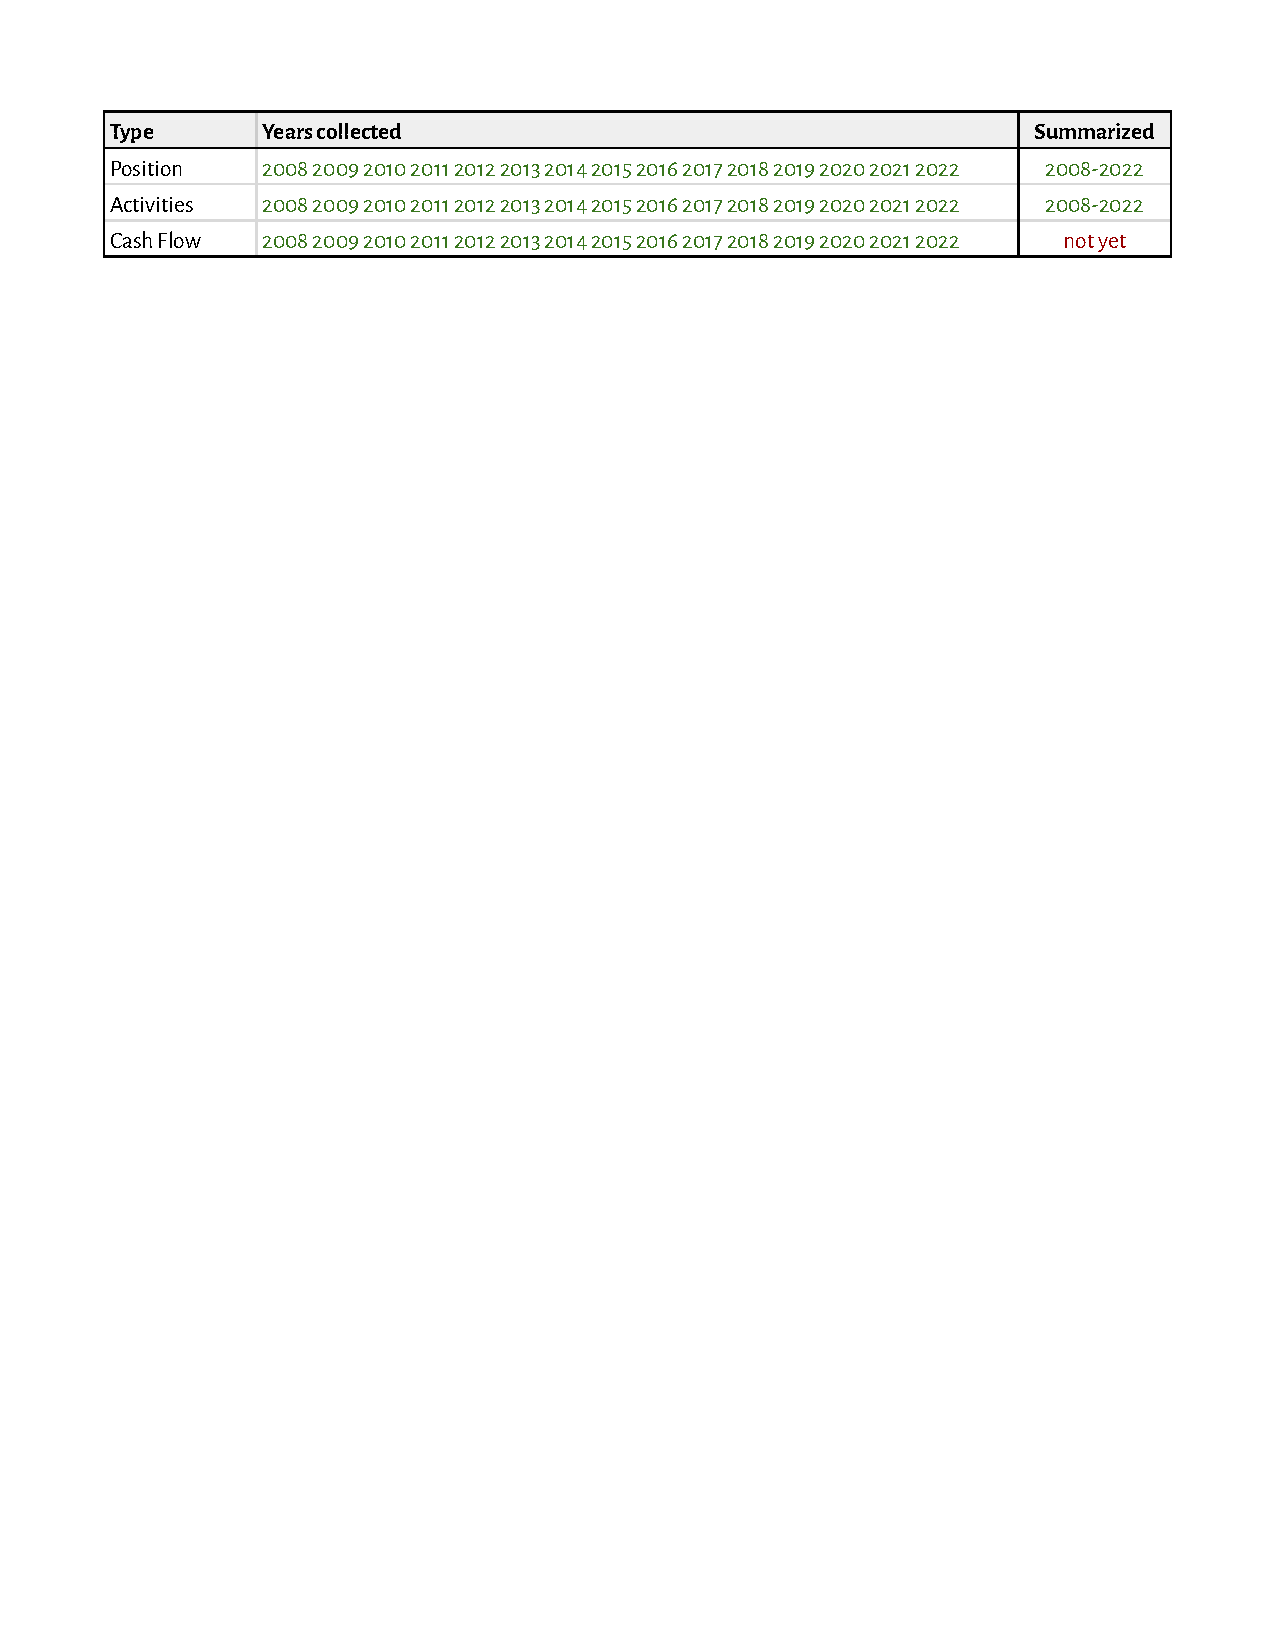
\includegraphics[page=1,width=\textwidth]{Financial_Statements_Collected}
\end{figure}

\subsection{Debt}\label{sec:debt}



\subsubsection{Petitions \& Renewals}\label{sec:petitions-renewals}\indent

The current number of pages of initial and renewal petitions runs to 7371 pages for just Rocketship schools in Santa Clara County.\footnote{The massive size of some of these petition calls into question whether authorizers read them in their entirety.}

\subsubsection{Authorizer Staff Reports}\label{sec:findings-authorizer-staff-reports}\indent

\subsubsection{Budgets, Interim Reports, and CAFRs}\label{sec:findings-budgets-etc}\indent

\subsubsection{LCAPs}\label{sec:findings-lcaps}\indent

\subsubsection{Board and Committee Supporting Material}\label{sec:findings-board-material}\indent

\subsection{Facilities Options}\label{sec:findings-facilities-options}\indent

\subsubsection{Co-Locating}\label{sec:findings-co-locating}\indent

\subsubsection{Leasing}\label{sec:findings-leasing}\indent

\subsubsection{Owning}\label{sec:findings-owning}\indent

\subsection{Funding Facility Ownership}\label{sec:findings-funding-ownership}\indent

\subsubsection{Private Funding, Loans, and Foundation Grants}\label{sec:findings-private-funding}\indent

\subsubsection{Venture Funds}\label{sec:findings-venture-funds}\indent

\subsubsection{Tax Credits}\label{sec:findings-tax-credits}\indent

<<<<<<< HEAD
=======
\subsection{Tax Credits}\label{sec:tax-credit}\indent

>>>>>>> 4685233 (Fixups to 'methods.tex'.)
The New Market Tax credit of 39\% (5\% for the first 3 years, and 6\% for the remaining 4 years) can be applied to taxes due from other investments. Since there is a compounding effect, the 39\% is actually worth over 41\% of the initial investment. Note that these other investment may themselves have a return. With these kinds of incentives, it's no wonder that the New Markets Tax Credit is popular. But one should not be deceived into thinking that just because New Markets Tax Credits must be made in economically depressed area that investors are investing out of the goodness of their heart. The tax credit investment is nearly without risk because the tax credit is guaranteed as long as the charter school remains open. If the school stays open for seven years, the risk is zero.

\subsubsection{Bonds}\label{sec:findings-bonds}\indent

 Three bond prospectuses total over 1000 pages.    

% \subsection{Real Estate Data}\label{sec:real-estate-data}\indent
% \begin{enumerate}
%   \item What is the actual price, date, and buyer \& seller information for each property?
%   \item What is the legal relationship between Rocketship Education and Launchpad Development?
%   \item How were Rocketship facilities in Santa Clara County financed?
%   \item What are the type and terms of all bonds.
%   \begin{enumerate}
%     \item What bonds were floated: type, rate, \& terms; guaranteed by whom or how? If the bonds are not privatedly placed, they are classed as securities, and their prospectuses are filed with the Securities Exchange Commission and are publicly viewable.
%     \item For conduit bonds, the California Department of Education or Department of Finance web sites 
%   \end{enumerate}
%   \item Enumerate all known leases and their terms. Was part of the lease payment paid by California?
%   \item Enumerate all known loans.
%   \begin{enumerate}[a.]
%     \item What was used as collateral? 
%     \item What were the terms?
%   \end{enumerate}    
%   \item Enumerate donations from foundations and individuals.
%   \item Enumerate venture fund investments.
% \end{enumerate}


% Forms which have been filed with a government entity:
%  \begin{enumerate}
%   \item Federal 990 forms to check against financial statements. IRS maintained. Should cross-reference the financial statements.
%   \item Annual and interim budgets submitted to the California Department of Education.
%   \item Petition approvals and renewals submitted to local school districts, the SCCOE, or the California State Board of Education.

%   The Santa Clara County Office of Education (SCCOE), and each school district in which Rocketship petitioned to open a school has some data/notes from one or more board meetings in which the petition or renewal was discussed. These data might have been presented by Rocketship or by county or district staff. Sometimes there is also public comment.
  
% Often, petitions presented to a school district have been denied and appealed to the Santa Clara County Board of Education, and in a few cases, to California's State Board of Education.
  
%   \item There is some published material on Rocketship.
%   \begin{enumerate}[a.]
%     \item Some books have been written about Rocketship
%     \item Roxana has two ScoopIt collections on Rocketship on and charter schools.
%     \item The ``Stop Rocketship'' web site has lots of information on Rocketship.
%     \item Several academics have datasets of school or district financial information  which include Rocketship.
%     \item Numerous articles, web sites, and blog postings include Rocketship financial data.
%   \end{enumerate}
%   \item Other, outside entities that may add revenue to Rocketship
%   \begin{enumerate}
%     \item Zeal
%     \item Dreambox Learning
%   \end{enumerate}
% \end{enumerate}


\section{Other Data}\label{sec:findings-other-data}\indent

\subsection{Datasets}\label{sec:findings-datasets}\indent

\subsection{State and Federal Filings}\label{sec:findings-state-federal-filings}\indent

\subsection{Curated Social Media}\label{sec:findings-curated-social-media}\indent


\section{Gaps and Anomalies}\label{sec:findings-gaps-anomolies}\indent

Since a goal of this dissertation is to map the flow of money into and out of Rocketship, I will use diagrams similar to the one used by \citeauthor{Baker.Miron2015} (\citeyear{Baker.Miron2015}), which is reproduced here as \prettyref{fig:opresflows}.

\subsection{Triangulation}\label{sec:findings-triangulation}\indent

These data represent the monies that are flowing into Rocketship/Launchpad related to facilities, real estate, bonds, loans, and donations and not tied to the number of students. Once that's been assembled, roll up into one spreadsheet, Rocketship's consolidated financial statements for the fourteen years (2008--2022). The consolidated financial statements can then be compared against the known real estate, bond, loan, and donation transactions. Noe where data is missing or where it conflicts with the consolidated financial statements.

\begin{figure}[ht]
  \centering
  \caption[Operating Resource Flows]{\textit{Operating Resource Flows}}\label{fig:opresflows}
  \includegraphics[width=\textwidth]{Operating_Resource_Flows}\\
  \footnotesize\raggedright\textcite[16]{Baker.Miron2015}.
\end{figure}
In this example, money flows from left to right, and there are no loops. Colors are used merely to distinguish the various blocks.

%%% Local Variables:
%%% mode: latex
%%% TeX-master: "Rocketship_Education-An_Exploratory_Public_Policy_Case_Study"
%%% End:
